\documentclass[tikz]{standalone}

\usepackage{tikz}
\usetikzlibrary{positioning, arrows.meta, calc}

\begin{document}

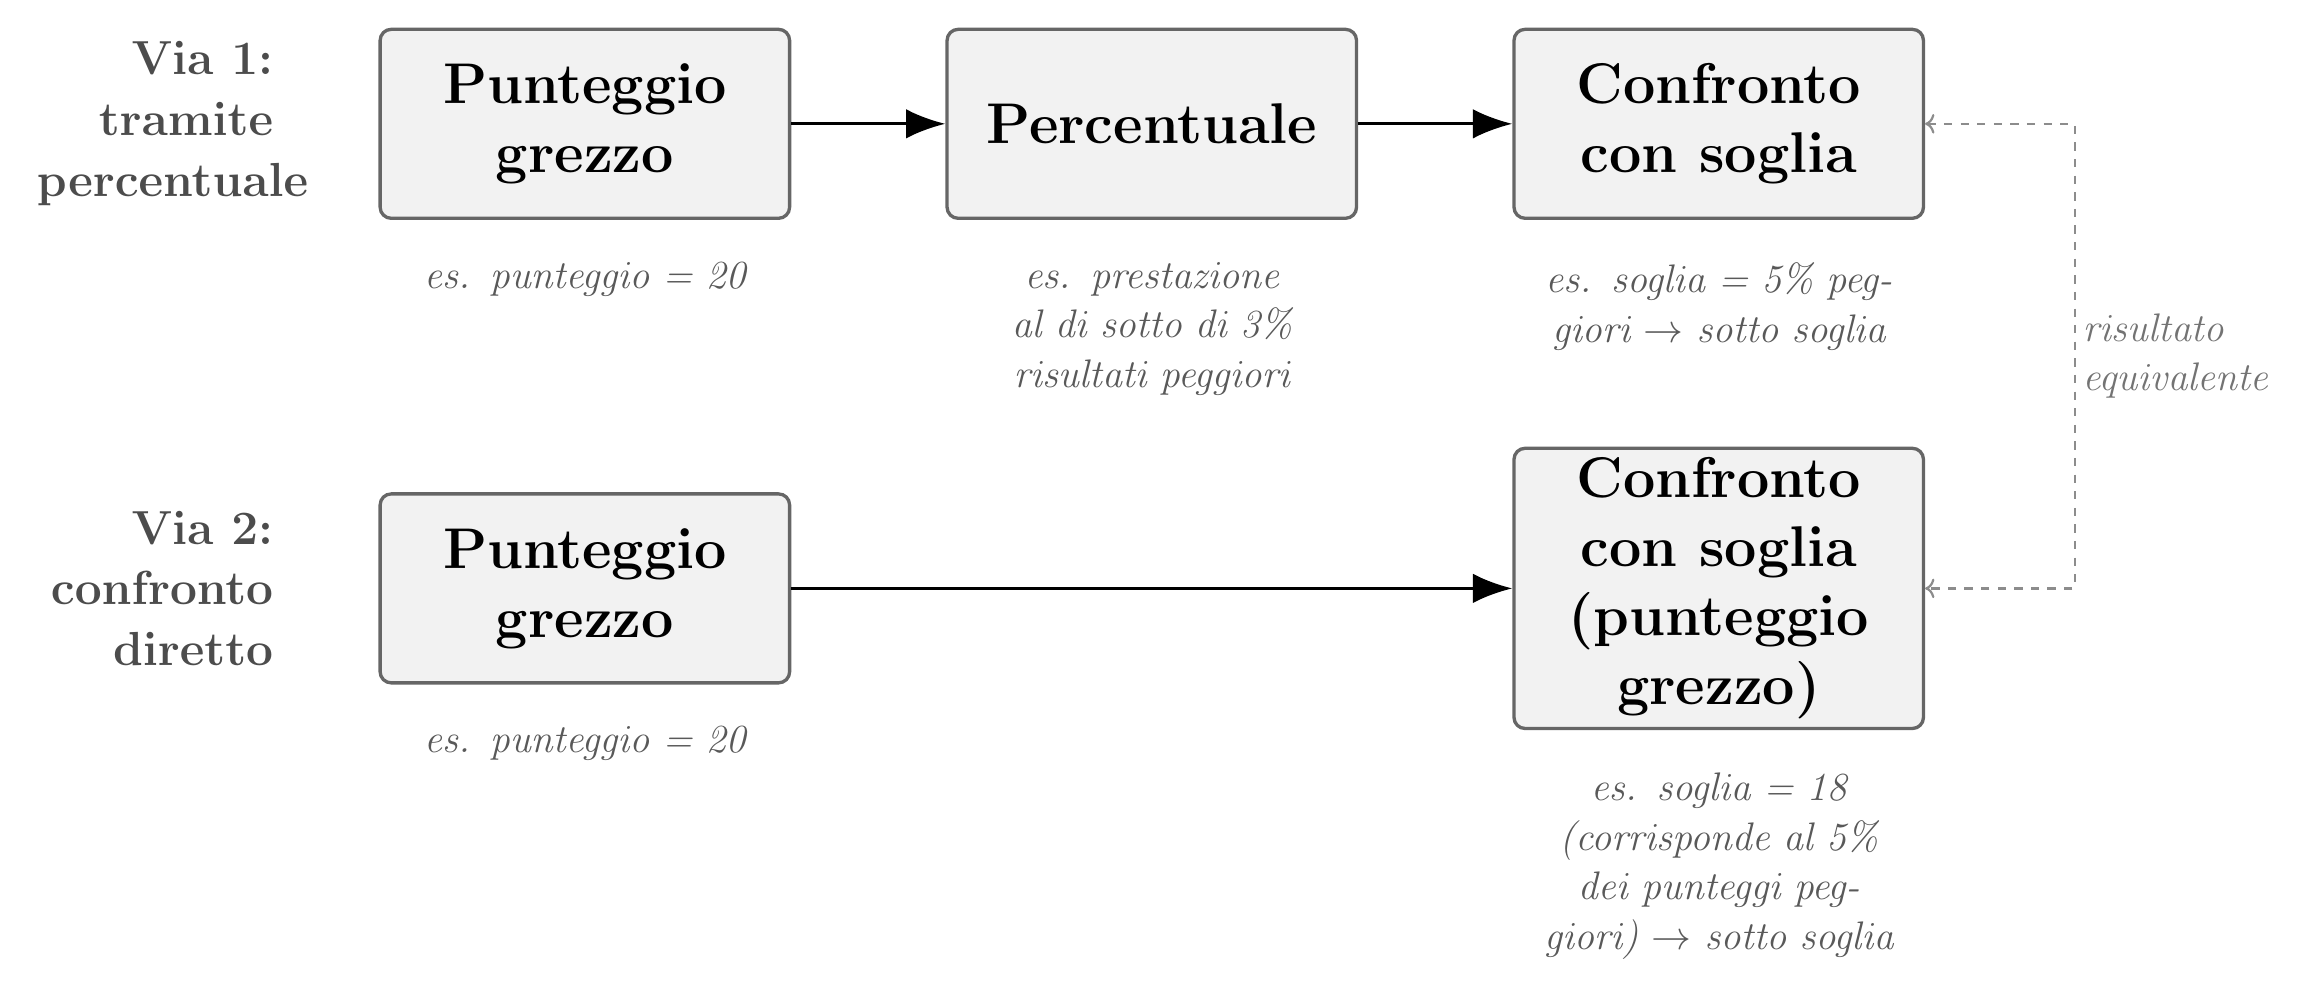
\begin{tikzpicture}[
    every node/.style={font=\LARGE},
    very thick,
    block/.style={
        draw=black!60,
        fill=black!5,
        rounded corners,
        minimum width=5.2cm,
        minimum height=2.4cm,
        text width=4.8cm,
        align=center,
        font=\huge\bfseries
    },
    example/.style={
        text width=4.6cm,
        align=center,
        font=\Large\itshape,
        text=black!65
    },
    rowlabel/.style={
        font=\LARGE\bfseries,
        text=black!70,
        align=right,
        text width=3cm
    }
]

% --- Riga sopra: via del percentile ---
\node[block] (A1) at (0,0) {Punteggio grezzo};
\node[block] (A2) at (7.2,0) {Percentuale};
\node[block] (A3) at (14.4,0) {Confronto con soglia};

\node[example, below=0.4cm of A1] (A1ex) {\textit{es. punteggio = 20}};
\node[example, below=0.4cm of A2] (A2ex) {\textit{es. prestazione al di sotto di 3\% risultati peggiori}};
\node[example, below=0.4cm of A3] (A3ex) {\textit{es. soglia = 5\% peggiori $\rightarrow$ sotto soglia}};

\draw[-{Latex[length=5mm]}] (A1) -- (A2);
\draw[-{Latex[length=5mm]}] (A2) -- (A3);

\node[rowlabel, left=1.2cm of A1] (labelA) {Via 1:\\ tramite\\ percentuale};

% --- Riga sotto: via del confronto diretto ---
\node[block] (B1) at (0,-5.9) {Punteggio grezzo};
\node[block] (B2) at (14.4,-5.9) {Confronto con soglia\\ (punteggio grezzo)};

\node[example, below=0.4cm of B1] (B1ex) {\textit{es. punteggio = 20}};
\node[example, below=0.4cm of B2, text width=6.2cm] (B2ex) {\textit{es. soglia = 18\\ (corrisponde al 5\% dei punteggi peggiori) $\rightarrow$ sotto soglia}};

\draw[-{Latex[length=5mm]}] (B1) -- (B2);

\node[rowlabel, left=1.2cm of B1] (labelB) {Via 2:\\ confronto diretto};

% --- Collegamento di equivalenza tra le due vie (instradato a destra, per non attraversare i testi) ---
\coordinate (eq1) at ($(A3.east)+(1.9,0)$);
\coordinate (eq2) at (eq1 |- B2.east);
\draw[<->, dashed, thick, color=black!45]
    (A3.east) -- (eq1) -- (eq2) -- (B2.east);
\node[font=\Large\itshape, text=black!55, align=left, text width=2.4cm] at ($(eq1)!0.5!(eq2)$) [xshift=1.3cm] {risultato equivalente};

\end{tikzpicture}

\end{document}
